\documentclass[12pt]{book}
\usepackage[explicit]{titlesec}
\usepackage{lmodern}
\usepackage{lipsum}
\let\cleardoublepage\clearpage
\newlength\chapnumb
\setlength\chapnumb{4cm}

\titleformat{\chapter}[block]
{\normalfont\sffamily}{}{0pt}
{\parbox[b]{\chapnumb}{
   \fontsize{120}{110}\selectfont\thechapter}
  \parbox[b]{\dimexpr\textwidth-\chapnumb\relax}{
    \raggedleft
    \hfill{\LARGE#1}\\
    \rule{\dimexpr\textwidth-\chapnumb\relax}{0.4pt}}}
\titleformat{name=\chapter,numberless}[block]
{\normalfont\sffamily}{}{0pt}
{\parbox[b]{\chapnumb}{
   \mbox{}}
  \parbox[b]{\dimexpr\textwidth-\chapnumb\relax}{
    \raggedleft
    \hfill{\LARGE#1}\\
    \rule{\dimexpr\textwidth-\chapnumb\relax}{0.4pt}}}
   
\usepackage[a4paper,top=2cm,bottom=2cm,left=2cm,right=2cm]{geometry}
\usepackage[T1]{fontenc}
\usepackage[utf8]{inputenc}
\usepackage{graphicx}
\usepackage{afterpage}
\graphicspath{{images/}}
\usepackage[english,italian]{babel}
\usepackage{hyperref}
\usepackage{lscape}

\setcounter{tocdepth}{2}


\title{DESIGN DOCUMENT document}
\author{Alessandro Negrini \and Andrea Gulino \and Paolo Guglielmino}
\date{October 2014}

\begin{document}
\selectlanguage{english}

\tableofcontents
\afterpage{\null\newpage}

\chapter{Introduction}

In this phase of software development, we have to provide conceptual idea of our software design. We will also provide the software architecture, system specification, error handling specifications which are primarily supposed to be implemented. \\
We think that the right way to proceed is to use design and architectural patterns, that allows us to reuse the code and resolve frequent problems in a smart and efficient way. \\

\section{Refactoring RASD}

Due to some internal issues within Design and Implementation of Mobile Application and time constraints, we won't developed the mobile application of this software as expressed in the RASD Document. So this system will be accessed only through a web application. However, this does not mean that the application cannot be used in a mobile device,in fact we will build a responsive user interface that will easily fit the mobile device browser. \\

In addition, we also performed some other updates in the Class Diagram part. 
We deleted the class Calendar from the UML Class Diagram ( the reason why we made it is explained further ). 
Some other minor changes are represented by the fact that weatherForecast Class is associated to Event Class, instead of Location one. \\
Finally, we add two attributes to the class User: avatar and info, in order to provide more information about the user, like common in social applications. \\
Anyway, in the next page we provide the up to date Class Diagram in order to be more clear. 

\newpage
\begin{landscape}
\begin{center}
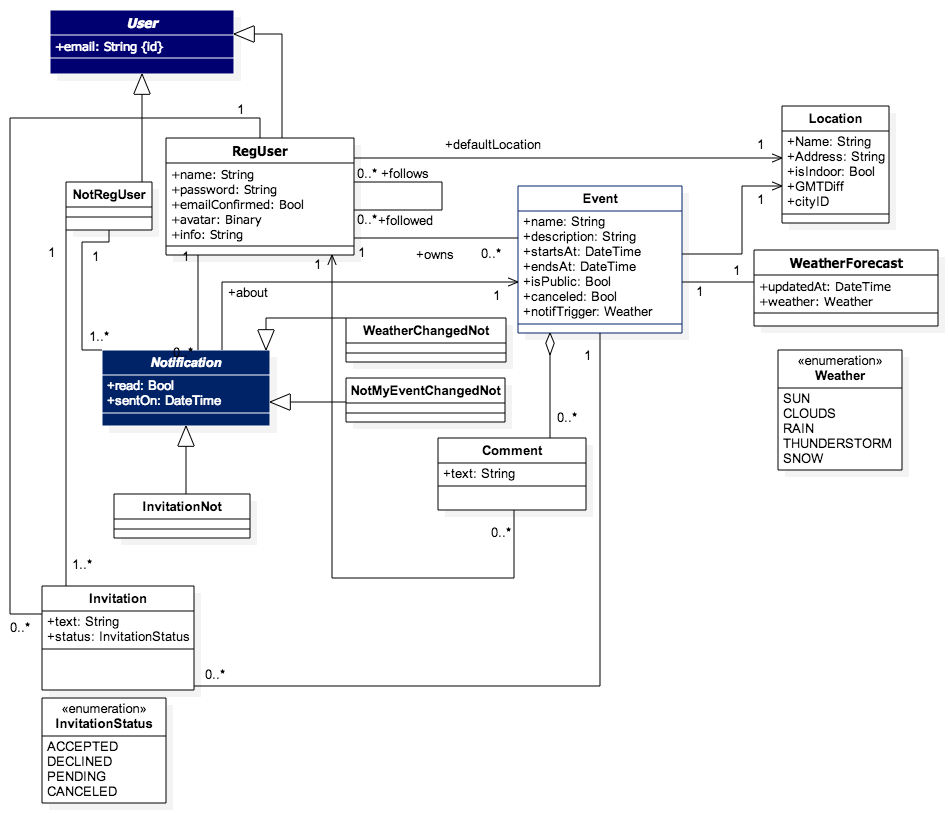
\includegraphics[scale=0.57]{class_diagram}
\end{center}
\end{landscape}

\section{Purpose}
The Software Design Document is a document that provides documentation which will be used to support software development by providing the details on how the software should be built. It will be our overall guidance during the entire development, under the architectural and design point of view. It is addressed not only to the team members, but also to external people allowing them to understand what it will be built and how it is expected to be built. \\
With respect to the RASD Document, DD will be a little more technical, in fact it is addressed to competent users, like team developers and also analysts. This stakeholders' heterogeneity is taken into account. \\
DD is based on many formal diagrams, such as UX diagrams, ER Diagrams, BCE Diagrams and Sequence Diagrams. \\
However, every diagram is accompanied with a narrative description in order to explain things also in a textual way, that sometimes can be more clear for non-technical people. \\

\section{Intended Audience}
The intended audience of this document is the following: \\

\textbf{Project Team: } DD is the guideline and reference of the software design and architecture  for the team members during the development and the maintaining process. \\

\textbf{Supervisors: } DD gives an overview of the software design and architecture, explaining which patterns were used during development. 

\section{Definitions, acronyms, abbreviations}
Listed below are some definitions of those terms used inside the document that may cause ambiguity. \\ \medskip

\begin{tabular}{ |l|l| }
  \hline
  \hline
  \multicolumn{2}{|c|}{\large{\textbf{Dictionary}}} \\
  \hline
  \hline
  \textbf{Keyword} & \textbf{Definition} \\
  \hline
  \textbf{Supervisors} & In this project teachers and tutors are considered supervisors of the \\&project\\
  \textbf{Tier} & system physical subdivision\\
  \textbf{Layer} & system logical subdivision\\
  \textbf{Principals} & user who has been authenticated by an authentication system\\
  \textbf{Role} & users are collected into groups, called roles\\

  \hline
  \hline
\end{tabular} \\ 
\vspace{0.5cm}

In addition we think that it can be useful to make a glossary of abbreviations and acronyms:  \\ \medskip

\begin{tabular}{ |l|l| }
  \hline
  \hline
  \multicolumn{2}{|c|}{\large{\textbf{Glossary}}} \\
  \hline
  \hline
  \textbf{Acronym or Abbreviation} & \textbf{Definition} \\
  \hline
  \textbf{DD} & Design Document\\
  \textbf{RASD} & Requirements Analysis and Specification Document\\
  \textbf{BCE} & Boundary Control Entity \\
  \textbf{UX} & User eXperience\\
  \textbf{JEE} & Java Enterprise Edition\\
  \textbf{EJB} & Enterprise Java Beans\\
  \textbf{JPA} & Java Persistence API\\
  \textbf{ORM} & Object-Relational Mapping\\
  \textbf{JPQL} & Java Persistence Query Language\\
  \textbf{JSP} & Java Server Page\\
  \textbf{JSF} & Java Server Faces\\
  \textbf{DBMS} & DataBase Management System\\
  \textbf{MVC} & Model-View-Control\\
  \textbf{IDE} & Integrated Development Environment \\
  \textbf{SMTP} & Simple Mail Transfer Protocol\\
  \textbf{API} & Application Programming Interface\\
  \textbf{JAAS} & Java Authentication and Authorization Service\\

  \hline
  \hline
\end{tabular} \\

\section{Overview}

The Software Design Document is divided into 10 chapters with various subsections.\\

These are : 
\begin{itemize}
\item{\textbf{System Overview: }} in this part we give a brief description of the system, presenting a first idea of architecture. Then technologies and tools used are listed
\item{\textbf{System architecture: }} a more detailed architecture description is given. In this chapter we show how the JEE architecture will influence our software development. 
Finally, we will provide a detailed description of each considered layer. 
\item{\textbf{Persistent Data Management: }} this part concerns with designing the conceptual and the logic diagram. 
\item{\textbf{Human Interface Design: }}User eXperience adds the process and techniques necessary to design and build a user interface that will meet requirements and allow users to exercise all the system behaviour described in use cases. 
\item{\textbf{BCE Diagrams: }}in this section we subdivide the application into three components, Boundaries, Controllers and Entities and then they are modelled stereotipying Class Diagrams. So it will given a static view of the application taking care of this subdivision of components. 
\item{\textbf{Sequence Diagrams: }}in this part we will provide a set of sequence diagrams ( not all the possible ones, but just the most important). They are derived from BCE diagrams. So with respect to the ones inside the RASD Document, they're more detailed because we will show how Boundary Controller and Entities works in dynamic way
\item{\textbf{Used tools }} 
\item{\textbf{References }}
\end{itemize}

\chapter{System Overview}
This part is intended to provide a brief overview of the systesm. We will explain the main logical components of the system looking at them from an high abstraction level and show relations among them. \\
As most of applications, our software is composed by the front-end part, for user interaction (client),  and the back-end one (server), for business logic and data management. 
Further, a more detailed tier division will be given, here we give just a rough idea. \\ The general scheme can be seen as the following well known client-server architecture: \\
\begin{center}
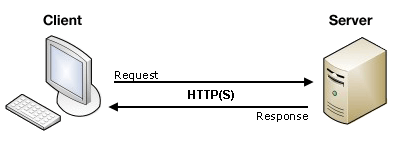
\includegraphics[scale=0.7]{client-server}
\end{center}
Above just one client is represented, but our system can support more than one client, theoretically an infinite number, depending on the capabilities of the server. 

\section{Technological Environment}
In the next chapter, we will start analyzing the system architecture in a detailed way and discussing the reasons why we adopted a solution rather than another. \\ 
Since some architectural choices we took are dependent from the specific technology used, we want to point out technologies and tools we used. \\
However, the technological choices we took, take care of constraints imposed by supervisors and they are based on JEE platform. \\

The system is based on JEE 7. In particular we will use these services : 
\begin{itemize}
\item{Enterprise JavaBeans (EJB) for server side logical business  }
\item{Java Persistence API (JPA) : Standard API for object-relational mapping (ORM). With Java Persistence Query Language (JPQL) we can query objects stored in the database}
\item{JavaMail:  our system requires the ability to send emails}
\item{JavaServer Pages(JSP), JavaServer Faces(JSF) and Servlet for the web tier }
\item{JEE implementation is provided by application server GlassFish, version 4.1}
\item{DataBase Management System (DBMS) used is MySql Community Edition version 5.5. However, this choice is not critical, in fact database server communication is abstracted by JPA. \\ Substituting MySql with others, like Derby, Postgres, ... will not imply code updates. }
\item{OpenWeatherMap as weather API that sends weather forecasts to our system as JSON/XML document}
\item{As for IDE, we use NetBeans that is more prone to JEE application development }
\item{The structure of the project is based on Maven (that's make the structure, compilation and the deployment standard and allows to get a project more portable and independent from the platform)}
\item{JUnit as framework to write and run repeatable tests. }
\item{Finally, as distributed version control system we use Git and Google Code as remote repository }
\end{itemize}

\chapter{System architecture}

The architectural style we adopted, multi-tier, is the usual for enterprise applications, where different layers are distributed on different physical devices (tiers) that communicate through web. \\
Before starting explaining our application's architecture we want to focus on JEE Architecture, the one we adopt to carry out the system development.\\

Although sometimes terms 'tier' and 'layer' are used as synonyms, we want to clarify that when we use 'layer' we are referring to the system logical division. Instead, using 'tier' we report to system physical division. 
\begin{center}
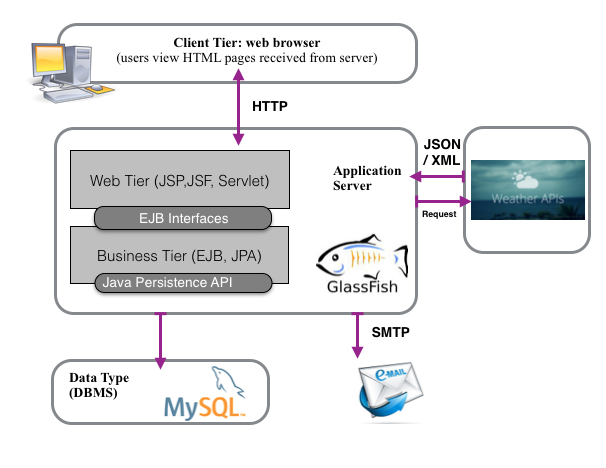
\includegraphics[scale=0.7]{jee}
\end{center}

\section{Security}
In the RASD Document when we dealt with non functional requirements we stated that our most important requirement was the security and the privacy part. \\
Therefore, now we would like to spend some words about this topic and how we will use JEE in order to satisfy it. \\
When we use the word 'security' we can refer to many concepts. It can go from securing a network, to encrypting data transfer, to granting users certain permissions on a system. In particular we will focus on authentication and authorization. \\
JEE has defined several mechanisms to secure applications and we will use some of them. \\
In our application will be important concepts like 'Principal' and 'Role'. A principal represents a user who has been authenticated by an authentication system. When a principal is given to a user, he must be organized into a specific group of user. The following figure shows how users can be represented in a secure system : 
\begin{center}
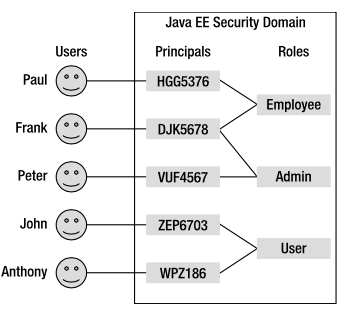
\includegraphics[scale=0.6]{principals}
\end{center}

In our application we will focus on three important aspects: authentication, authorization and data cryptography. 
As already told, authentication is the process of verifying the user's identity ( in our application this can be verified using a username and password verification) and assigning a principal to the user. \\Authorization is the process of determining whether a principal has access to a particular resource or a function. Depending to his role, a user can have access to all resources, none or a subset. 
This figure shows a common security scenario, where user is asked to enter his username and password through a client interface and his credentials are checked using Java Authentication and Authorization Service (JAAS) against an underlying authentication system. JAAS is the API used internally by the web and EJB tier to perform authorization and authentication. 

\begin{center}
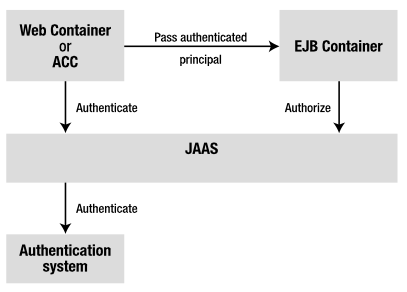
\includegraphics[scale=0.6]{aut_aut}
\end{center}

\section{Architectural Design}
MeteoCal architecture is divided in four logical levels (as JEE one): \textbf{Client Layer} (presentation), \textbf{Web Layer} and \textbf{Business Layer} (logic), \textbf{Data Layer}. 
\begin{itemize}
\item{\textbf{Client Layer: }} it is used by the user to access the application using an interface. In our specific case, since we will develop a web application, users do it through the web browser. On the other hand, if a simple Java Application would be developed, in the client layer we could have found instead of a web browser a specific client side Java Application. \\
In our web application, this layer communicates though HTTP protocol with the web layer, sending to server data provided by the user, and showing  HTML pages received. \\
In addition, the browser will interpret some piece of code written in JavaScript in order to improve the service and user experience (e.g asynchronous request to server for checking form data correctness, ... )\\
\item{\textbf{Web Layer: }} it contains Servlets and Dynamic Web Pages that need to be elaborated. It receives HTTP requests from client layer and it replies sending HTML pages eventually formatted. \\
These pages are generated depending on received data and by the interaction with the business layer, where there is the business logic. 
\item{\textbf{Business Layer: }} this level encapsulates business logic and it directly "speaks" with the stable memory where the database is stored. \\ The model of our application is represented by Entity Beans. The business logic and the database interaction are performed by EJB components. \\
In order to access the database, this layer is based on JPA, for ORM, abstracting the relational model into an object oriented model. \\
\item{\textbf{Data Layer: }} this module contains a DBMS that manages a database that allows data to be persistent. The server communicates with the database using the standard API specification JDBC.\\ In our application the database will be in the same physical machine of the server application, but it can live on its own on a different server, provided that it is linked through web with the application server. \\
\end{itemize}
Finally, it is expected to use a mail server to accomplish mail communications with users, both for account managing issues (confirmation, password reset) and for notifications. \\ So our business layer interacts with an external server (or an external service) using the SMTP protocol. \\

Such a system architecture, allows us to decouple views, control and model, following the so called 
MVC pattern.\\ Just to remember, the model refers to the domain specific representation of the information on which that application operates (in our architecture the Data Layer). \\
The Controller responds to events, typically user actions, and invokes changes on the model (the Business and Web Layers).\\
Finally, the View renders the model into a form suitable for interaction, typically a user interface element (the Client Layer).\\
Actually, this analogy between MVC and layers is not properly right. They act in a similar way, but are topologically different. \\
In fact, a fundamental rule of three-layer architecture is that presentation level doesn't communicate with the data one, but messages must pass through the intermediate level. Instead, the original MVC pattern is allowed to break this rule. \\
However, the way MVC and three layers divide levels is conceptually the same . 

As for tiers subdivision, typical architectures use two or three tiers to allocate the logical layers. \\
Considering the dimension of our project a two-tiered architecture could be a proper solution. Among the available two-tiers configurations, the one we could use would consider a 'thin client', that means that only the presentation layer is allocated on the client machine, and a 'fat server', where both logical and data layer are allocated. \\
During the development phase we simulate the interaction between client and server within the same machine. \\
\section{Decomposition Description}
As known there are three ways to proceed designing and developing a system, the top-down approach, the bottom-up approach and the mixed one. \\
A mix of bottom-up and top-down is normally used, in order to take the strength from both of the approaches. First we decided to adopt a bottom-up approach, in which elementary part of our system are individuated and specified in detail. Bottom up design will bring reusable components. \\
But in order to get a good structure we have to switch to the top down approach\\ 
The difficulty will be find a trade off between the two approaches.
However, in this part we will provide the subsystem division of our original system. We have drew a hierarchical tree diagram, where the root is the overall system and the leafs are the most elementary subsystems. \\

Subsystems we identified are : 
\begin{itemize}
\item{Sign up}
\item{Log in}
\item{User subsystems}
	\begin{itemize}
	\item{Event creation}
	\item{Invite Friends}
	\item{Event modification}
	\item{User profile}
		\begin{itemize}
		\item{Import/Export Calendar}
		\end{itemize}
	\item{Personal home page}
	\item{Social subsystem}
		\begin{itemize}
		\item{Search for a user}
		\item{Follow a user}
		\end{itemize}
	\item{Notifications}
	\end{itemize}
\item{Administrator panel}

\end{itemize}

\begin{landscape}
\begin{center}
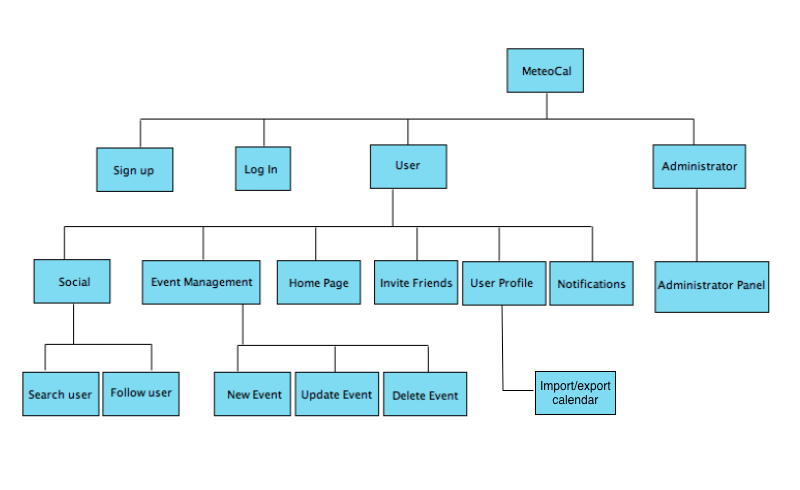
\includegraphics[scale=0.9]{subsystem}\\
\end{center}
\end{landscape}

\chapter{Persistent Data Management}
MeteoCal data layer is implemented using a MySQL DBMS that relies on a relation database.\\
In the following pages we will first present the conceptual design of our model, using the Entity-Relationship formalism, and then we will translate it into the logical model ending up with a concrete representation of the DB schema.\\
\section{Conceptual Design}
Conceptual design aims to give an abstract (semantic) representation of data used by the Application, independently from the database model (relational, OO, .. )\\
The ER conceptual model represents data in terms of entities and relationships between entities.\\
We decided to produce a unique ER diagram in order to provide a global and consistent view of the system data structure.\\

\newpage 
\begin{landscape}
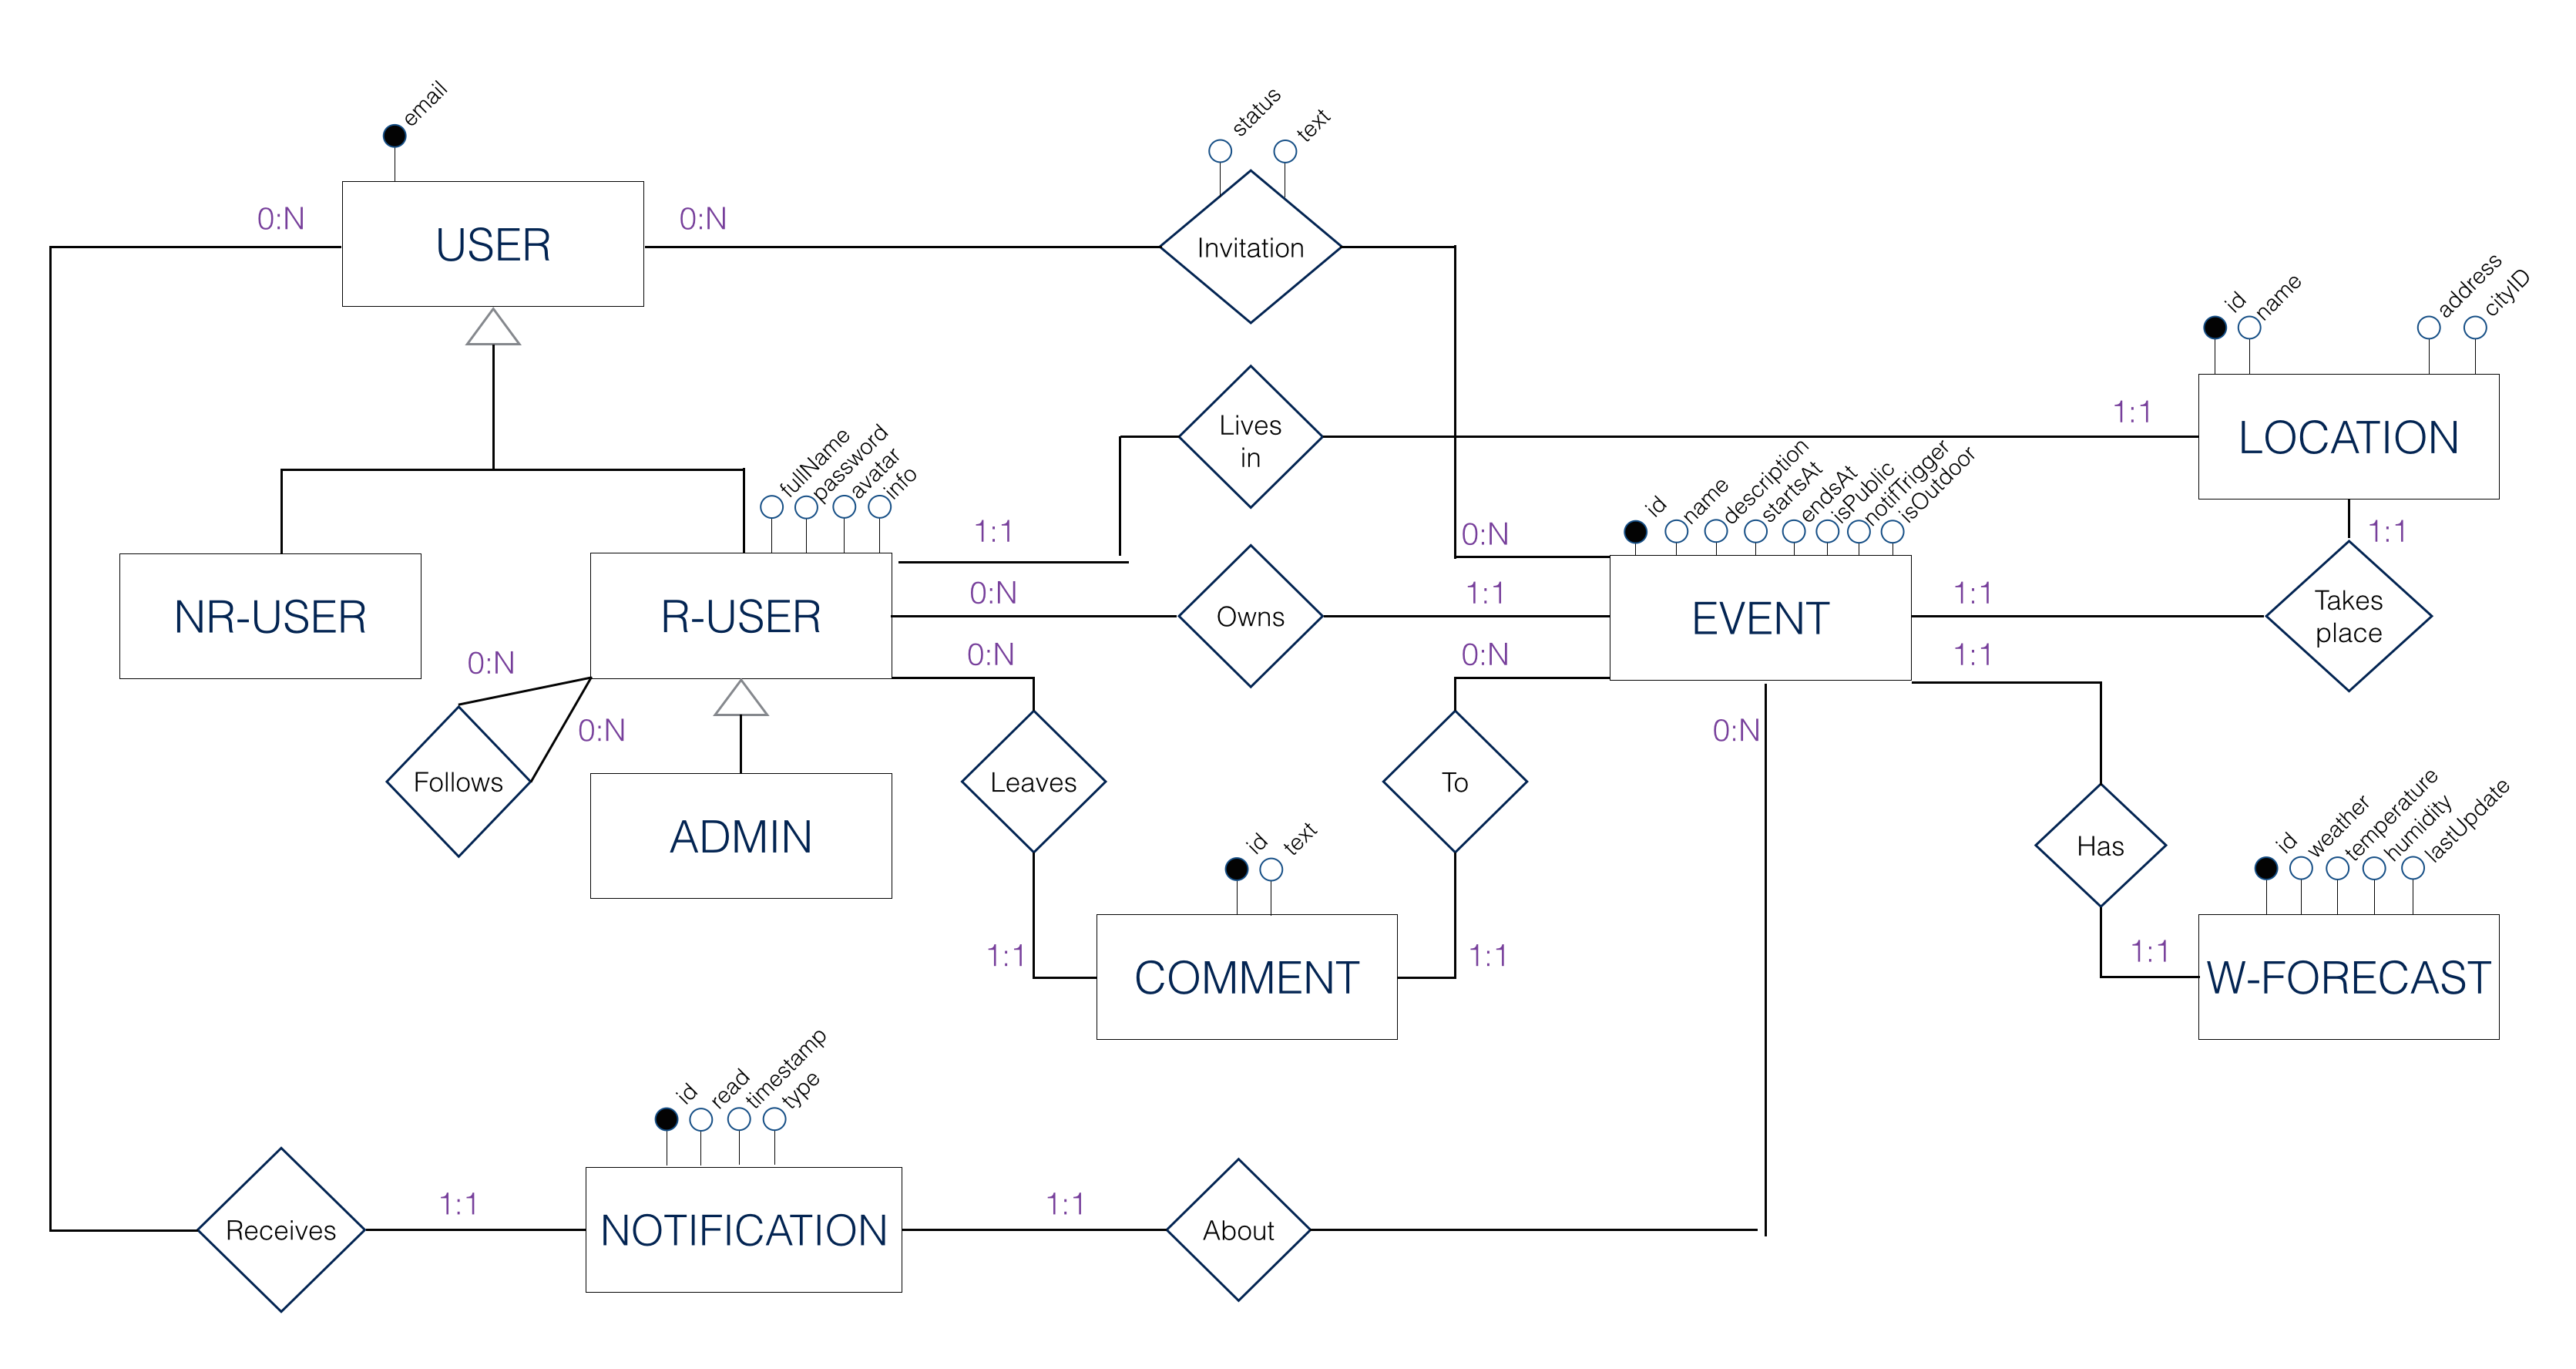
\includegraphics[scale=0.2]{er}\\
\end{landscape}

\section{Data Description}
\textbf{Users (entities USER, R-USER, NR-USER, ADMIN)}
In our application we make a distinction between three types of users: Registered Users (R-USER), Not Registered Users (NR-USER), and Administrators (ADMIN ).\\
Administrators have some additional capability with respect to Registered Users, and so they are represented through the entity ADMIN that is a sub-entity of R-USER.\\

We remind that a NR-USER is created when a R-USER invites a person, that is not registered to the system, to one of his events.\\
Its existence is therefore intended to keep memory of the invitations/notifications addressed to that person who will be able to manage them once registered to the system with the same email address.\\

All types of user are identified by their email address and inherit this key from the super-entity USER.\\

\textbf{Notifications (entity NOTIFICATION)}
A notification is a message automatically generated by the system when some user invites another user or when a change is detected on a event (weather change, date/time change, location .. )\\

We could have used another generalization to make a distinction between the different types of notification but it would have uselessly messed up the diagram.\\

Independently from the information they want to provide, notifications are all related to an EVENT and have the same attributes (a flag read indicating wether the notification has been read or not, a timestamp and a type indicating to the system what kind of information must be provided). \\
Note that using the attribute type  and the related EVENT the system can build the proper notification content (showing the new weather, the new date, and even redirecting to a received invitation), avoiding redundancies and inconsistencies.\\

\textbf{Locations (entity LOCATION)}
The concept of Location plays an important role within the application context and so it deserves to be described as an independent entity with a set attributes:\\
Name: to make the location easily identifiable by the user ('Home', 'School', .. )\\
Address: the street and civic number related to the location ('Jump Street 22', .. )\\
CityID: a number identifying the city; this attribute plays an important role in the process of weather forecast retrieval and time-zone inference.\\
The relation livesIn between R-USER and LOCATION is used to determine the time-zone according to which the event timing is displayed on the calendar and to provide information on current weather for that location.\\


\textbf{Weather Forecast (entity W-FORECAST)}
This entity is uniquely associated to an EVENT and represents a weather bulletin for the EVENT location at the EVENT time. \\
The attribute lastUpdate indicates the last time the system updated the weather bulletin.\\

\textbf{Events ( entity EVENT)}
We comment just the relevant attributes: \\
isPublic: a flag indicating the level of privacy associated to the event\\
isOutdoor: a flag indicating wether the event is indoor/outdoor\\
notifTrigger: weather condition to be satisfied (>=) in order to send weather notifications for outdoor events\\


\textbf{Invitations (relation INVITATION)}
Invitation is what links a User to an Event organized by a different user and has also the same meaning of a real-world invitation, that is why it is represented as a relation having two attributes: \\
text: a custom text provided by the inviter\\
status: an enumeration that can assume the values in (PENDING, ACCEPTED, DECLINED, CANCELED) representing the status of the invitation\\

\textbf{MeteoCal ... where's the Calendar?}
The Calendar is maybe the most important abstract entity of the whole application, but is it really necessary to model it as an independent entity?\\
The absence of an entity named Calendar answers the question, but why do we miss it?\\
A calendar is no more than a collection of events either created by the user or to which the user is invited (accepting the invitation), that have not been canceled.\\
The model we presented before contains all the sufficient information that is useful to reconstruct the user calendar! \\
In fact we can get the events created by the user from the relation CREATES, and the event to which the user will be a guest looking at the instances of the relation INVITATIONS having 'ACCEPTED' as status.
In addition we put the attribute  hasPublicCalendar  in R-USER to indicate wether the calendar is public or private.\\
Adding an entity Calendar would therefore mean adding redundancies (..waste of memory), and could cause inconsistencies, all things that is better to avoid.\\
\newpage

\section{Logical Design}
In this part of the document, the conceptual schema proposed above is translated into the logical one that corresponds with the real structure of our data in the DMBS\\
A logical data model describes the data in as much detail as possible, without regard to how they will be physical implemented by the DBMS.\\
Therefore the difference between Conceptual and Logical design is the level of detail we use to treat our data.\\
\subsection{ER Restructuration}
\begin{itemize}
\item{We merge the users hierarchy into a unique entity called User and we add an attribute called type to distinguish among the different types of user ('r-user', 'nr-user', 'admin')}
\end{itemize}
\subsection{Translation to Logical Model}
\begin{itemize}
\item{Relation Follows has cardinality 0:N on both edges so we create a new entity Follows with the two foreign keys followerEmail and followedEmail.}
\item{The same happens with relationship Invitation between User and Event, but in addition to the foreign keys sentTo and toEvent we add the relation attributes status and text}
\item{Comment has a many-to-one relationship with both User and Event, so we put two foreign keys inside Comment, one referring to User (leftBy) and one referring to Event (toEvent)}
\item{Event has a many-to-one relationship with User called Owns, so we include a foreign key named owner inside Event.}
\item{The same happens between Notification and User and between Notification and Event, in this case we add a foreign key referring to User named sentTo and another foreign key referring to Event named aboutEvent inside the entity Notification}
\item{Location  and Event are involved in a one-to-one relationship, we put a foreign key named location inside Event}
\item{We do the same with the one-to-one relationship between User and Location adding the foreign key livesIn inside User}
\end{itemize}

Below is drawn a graphical representation of the logical model:\\

\begin{center}
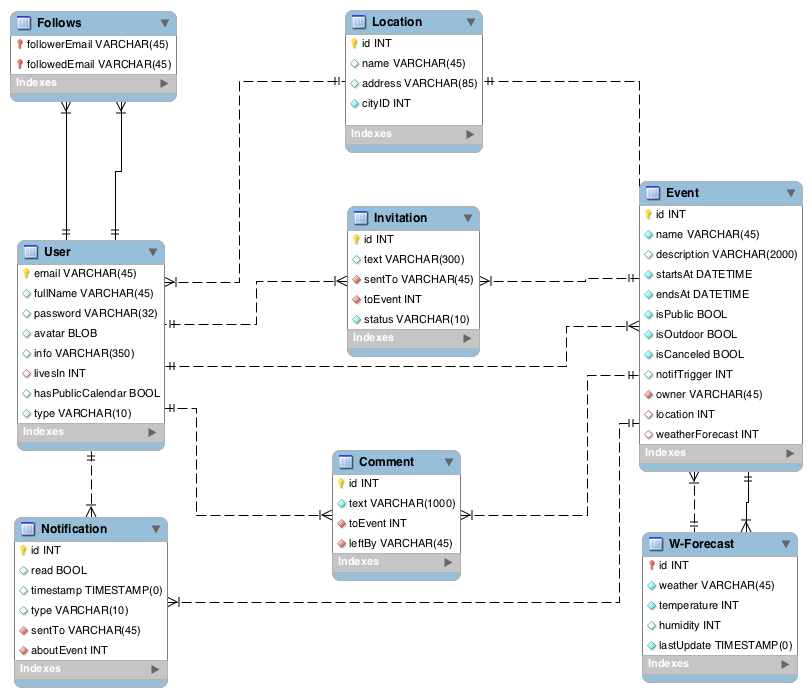
\includegraphics[scale=0.58]{logicalModel}\\
\end{center}
Finally, performing a direct mapping between the logical model entities and tables, we build the physical structure of data in our relational DB:\\

\textbf{User}( \underline{email}, fullName, password, avatar, info, \textit{livesIn}, hasPublicCalendar, type)\\

\textbf{Follows}( \underline{\textit{followerEmail, followedEmail}} )\\

\textbf{Event}( \underline{id}, name, description, startsAt, endsAt, isPublic, isOutdoor, isCanceled, notifTrigger, \textit{owner, location, weatherForecast})\\

\textbf{Invitation}( \underline{id}, text, \textit{sentTo, toEvent}, status)\\

\textbf{Location}( \underline{id}, name, address, cityID)\\

\textbf{Comment}( \underline{id}, text, \textit{toEvent, leftBy})\\

\textbf{Notification}( \underline{id}, read, timestamp, type, \textit{sentTo, aboutEvent})\\

\textbf{W-Forecast}( \underline{id}, weather, temperature, humidity)\\

Primary keys are underlined, foreign keys are written in italic.

\chapter{Human Interface Design}
Before concerning on the business layer, we want to focus on the web layer that deals with the user interaction.  
Thus, we described these functionalities using the User Experience (UX) diagram. UX diagrams are models that represent user interaction with the web application.\\
It is based on UML, so we use the Class diagram with appropriate stereotypes like \textit{<<screen>>}, \textit{<<screen compartment>>}, and \textit{<<input form>>}. \\
Screens are the list of screens that makes up the user interface, and they are related each other with associations which identify navigation paths. 
A screen may contain multiple input forms, each of it contains user input fields. In addition, they can contains also some screen components, that represent part of the page that can be shared with others. \\

In order to make our UX diagrams more understandable and readable, we have split our global system into some sub diagrams according to most important application functionalities. \\
Before starting to design UX diagrams, we wants to point out some important considerations : \\
\begin{itemize}
\item {UX diagrams designed below cover all the subsystems that we have indentified in chapter 3; }
\item{ it can happen that different UX diagrams, even if they deal with different part of the application, have some compartment or input forms in common.} 
\item {not all screen properties are necessary to be captured in the model. It is, after all, a simplification and an abstraction. Therefore, we won't design static content (label text and images) that are not architecturally significant. }
\item{ the static content is not appropriate to be the model}
\item {on the other hand dynamic content is an important elements of the UX model and it will be designed in the most clear way }
\end{itemize}
\section{Homes UX}
In this part, we have designed a UX Diagram that represents the different home pages, depending on the specific user is using the application. Our application is designed such that there can exists two kinds of users, the logged and the non-logged one. \\
Both home pages are inherited from the more generic Home screen marked with \$, this means that it can be reached from every page of the system. \\
This first diagram aims to give a global idea of the parts that shape the two kinds of MeteoCal homes, and for each compartment a principle of working is provided. \\
\subsection{UX description}
Our application starts with a home page as usual. \\
By default, the so called "not-logged User Home" will be shown as soon as a non-logged user accesses to it. Its goal is to provide users a way to log into the system or to create a new account. \\

If the users is not registered yet, he can sign up filling in the sign up form. When he is registered, or in case he is already registered, he can log into the application providing his credentials. \\
When he is logged in, the so called "Logged User Home" will be shown. 

This web page is composed by some compartments, such as : \\

- \textbf{Local weather compartment: }in this part daily weather forecasts are provided \\

- \textbf{User Options: }by it, users are allowed to logout or view profile info and also update them\\

- \textbf{Search Bar: }it allows to search for users by input their name \\

- \textbf{Notification Box: }it is a classical notifications container (like that used for Facebook notifications) in which the elements are organized from the most recent to the elder one. \\

- \textbf{Calendar: }this is the most important part of user home page. In fact, events are scheduled inside the calendar. We can have three different calendar views, by day, week or month. \\

- \textbf{Event Panel: }by it we can create a new event, and also have a overview of the most recent event  \\

Finally, user that logs into the system can be a system administrator and in that case, the administrator has the access to the application control panel that allows him to perform some modifications. \\
\newpage
\begin{landscape}
\begin{center}
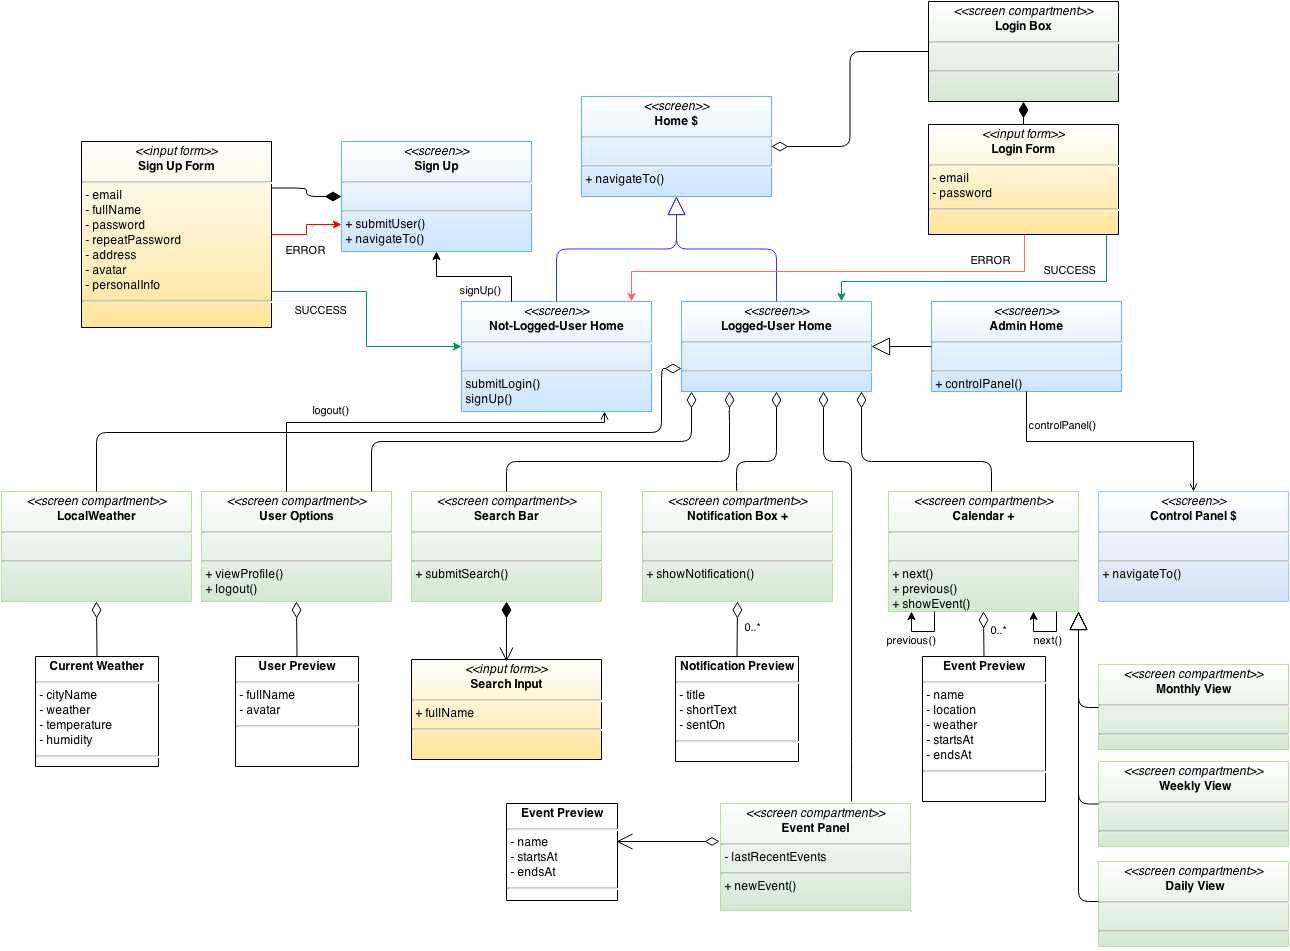
\includegraphics[scale=0.5]{homes_UX}\\
\end{center}
\end{landscape}

\section{Social functionalities UX}
This part of the document concerns with the functionalities that we call 'social', because they deals with typical operations of social networks, such as follow users and visit their public profile. 
\subsection{UX description}
In order to start following or visiting other users' profile, the user must first search for the target user using the search bar typing his name. A list of result is shown is a dynamic way. \\
By clicking on the profile that we want to visit, that user profile is displayed. 
The 'User Profile' screen is structured in a way that there' s a short description and the avatar of the user, that is the 'User Information' compartment and the 'Avatar' compartment. 
There is also the possibility to follow and unfollow (only in case in which the user is already followed) that user. \\
But, the main part of this screen is represented by the Calendar part, where the public calendar and the public events are displayed. In case in which the target user has made calendar public the scheduled is shown. 
On the other hand, if he decided to make it private, just an obscured compartment is displayed and there is no way to have a look to his scheduling.  
\begin{landscape}
\begin{center}
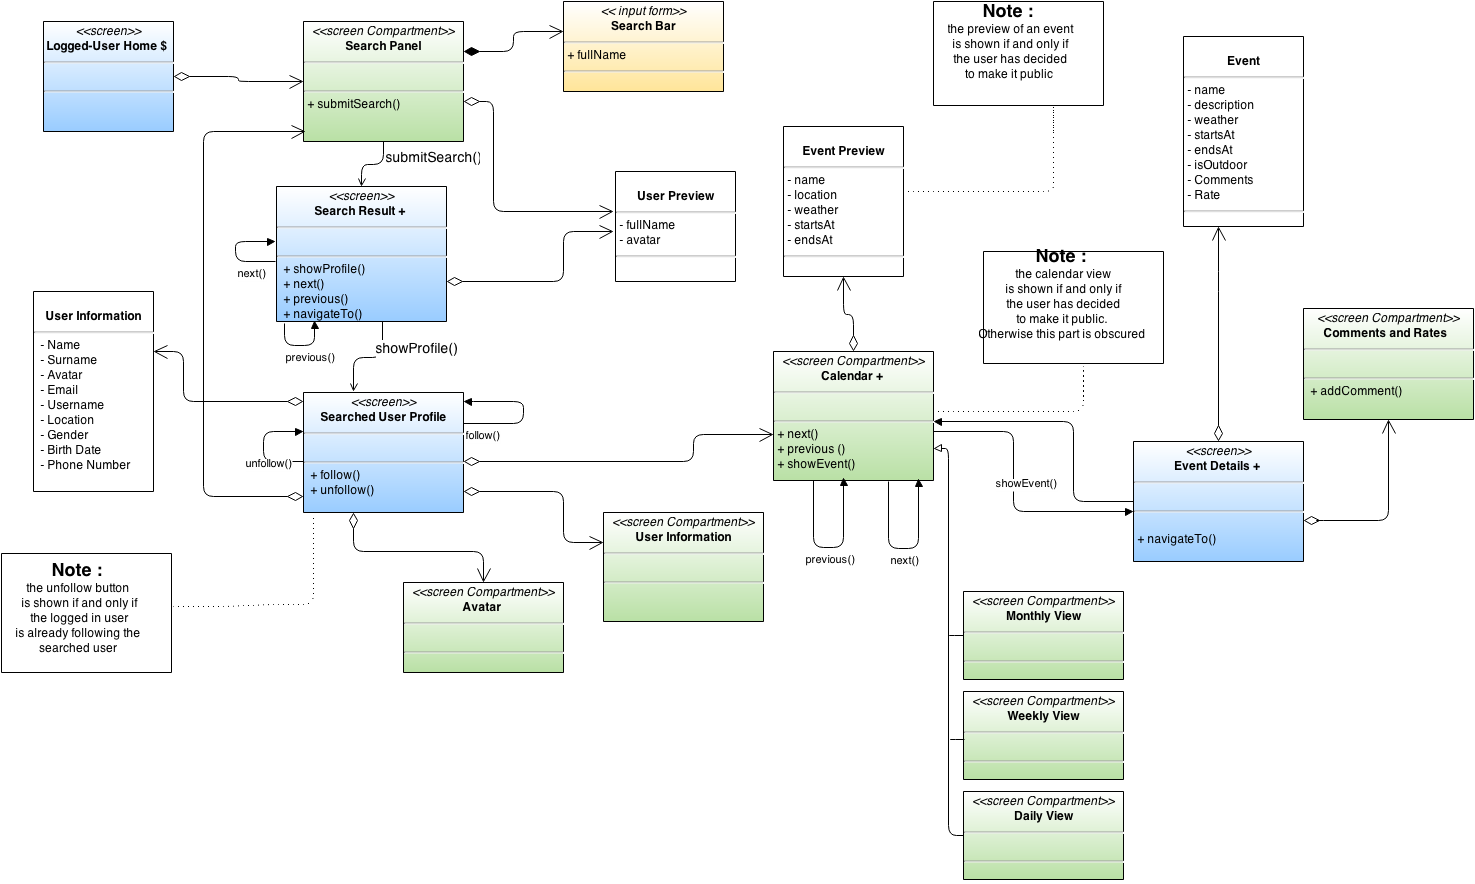
\includegraphics[scale=0.5]{social_UX}\\
\end{center}
\end{landscape}

\section{Profile Management UX}
From the option compartment, it is possible to get the access to his own profile and update information regarding account profile data, setting preferences about notifications, making calendar and events public or private and closing the account. 
\subsection{UX description}
From the 'user options' we can access our profile ('User Profile' screen) where user's information are collected and displayed. \\
Part of this screen is composed by some compartments that composed also the 'Logged User Home' screen, such as the search bar, the notification box. \\ 
In addition, user profile is structured in way that the user can upload, change and remove his avatar through the 'Avatar' compartment. Then he can have access to personal information. \\
By using this compartment user has the opportunity to update some account data (name, email, password, ... ). Then he can also set the visibility of his calendar, so choosing between public and private. \\
He can also set up some preferences about notifications, choosing in which case he wants to receive email notifications. \\
Finally, user have the opportunity to close his account. \\
In addition to these functionalities, through the notification box, the user can access the  notification subsystem, where a list of notifications (both past or pending) is shown. For pending notifications, he can also accept or refuse \\
\begin{landscape}
\begin{center}
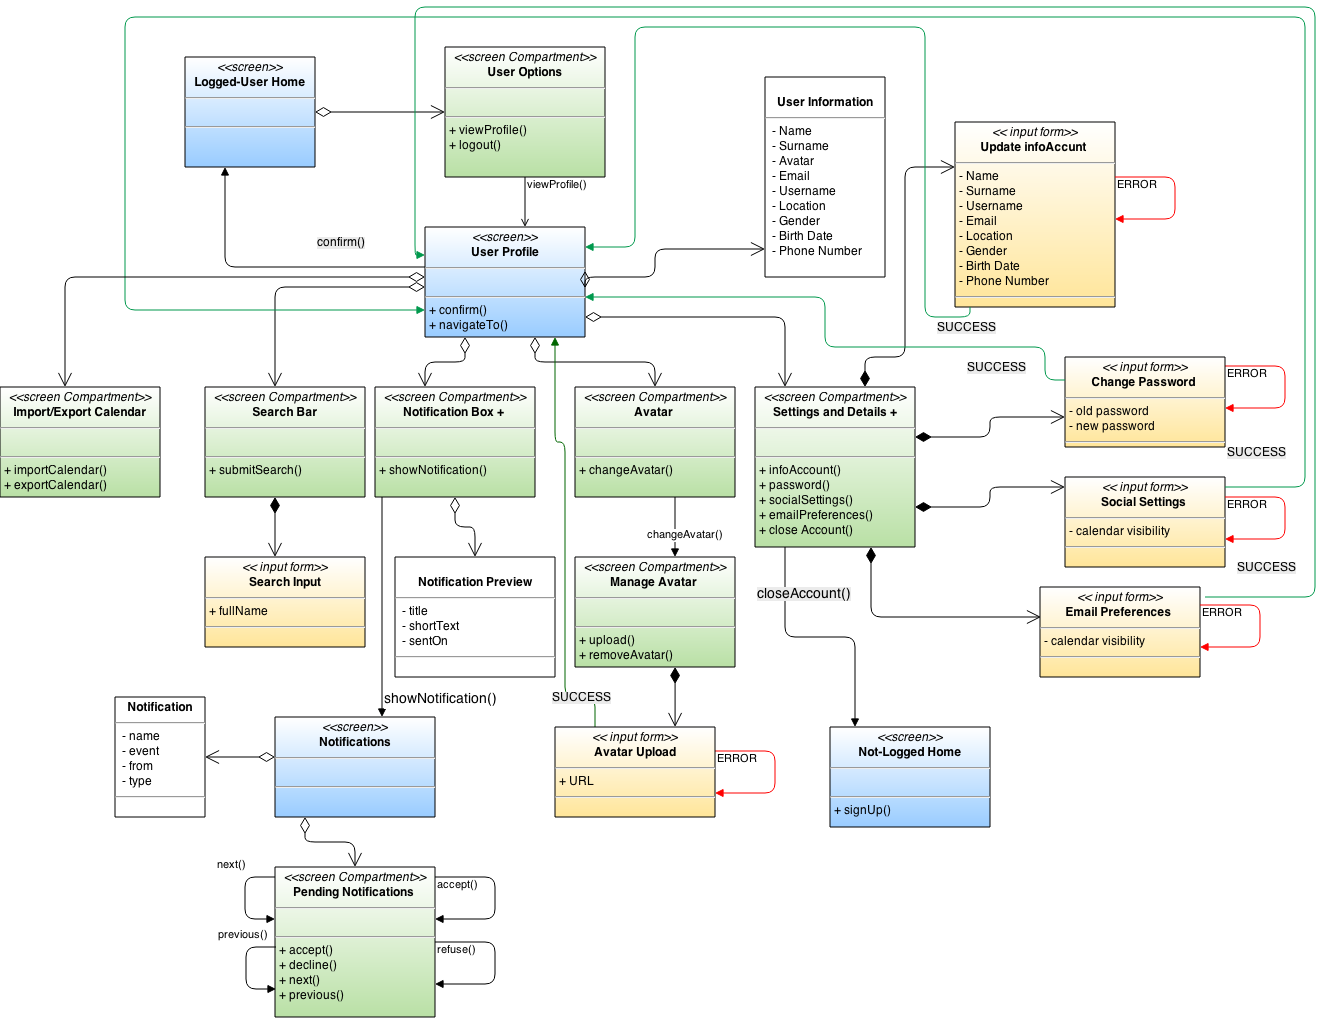
\includegraphics[scale=0.45]{profile_management_UX}\\
\end{center}
\end{landscape}

\section{Event Management UX}
This diagram describes the navigation flow about 'event management' process. With this name we refers to operations like the creation of a new event, the removal and the inspection of an existing event and the addition of friends to an event. 
\subsection{UX description}
This is the most important UX diagram because it shows how a user can create new events, can have a look on past events and scheduled events in the calendar, invite friends, and also can comment past events. \\
First, when a user wants to create a new event he has to fill in a form with all required info. During this process some errors can occur, like event conflicts with some other events, dateEnd(timeEnd) is less than dateStart(timeStart), and many others. \\ Through this compartment user can also have the opportunity to view the list of past events (events with dateEnd less than the current one) and for each of them take a look on details. For each event he can also add a comment it. \\
There is no way to invite friends to past events. \\
Instead, for events scheduled in the calendar that are not still performed, user can invite some friends using the proper 'invite Friends' form. \\ 
\newpage
\begin{landscape}
\begin{center}
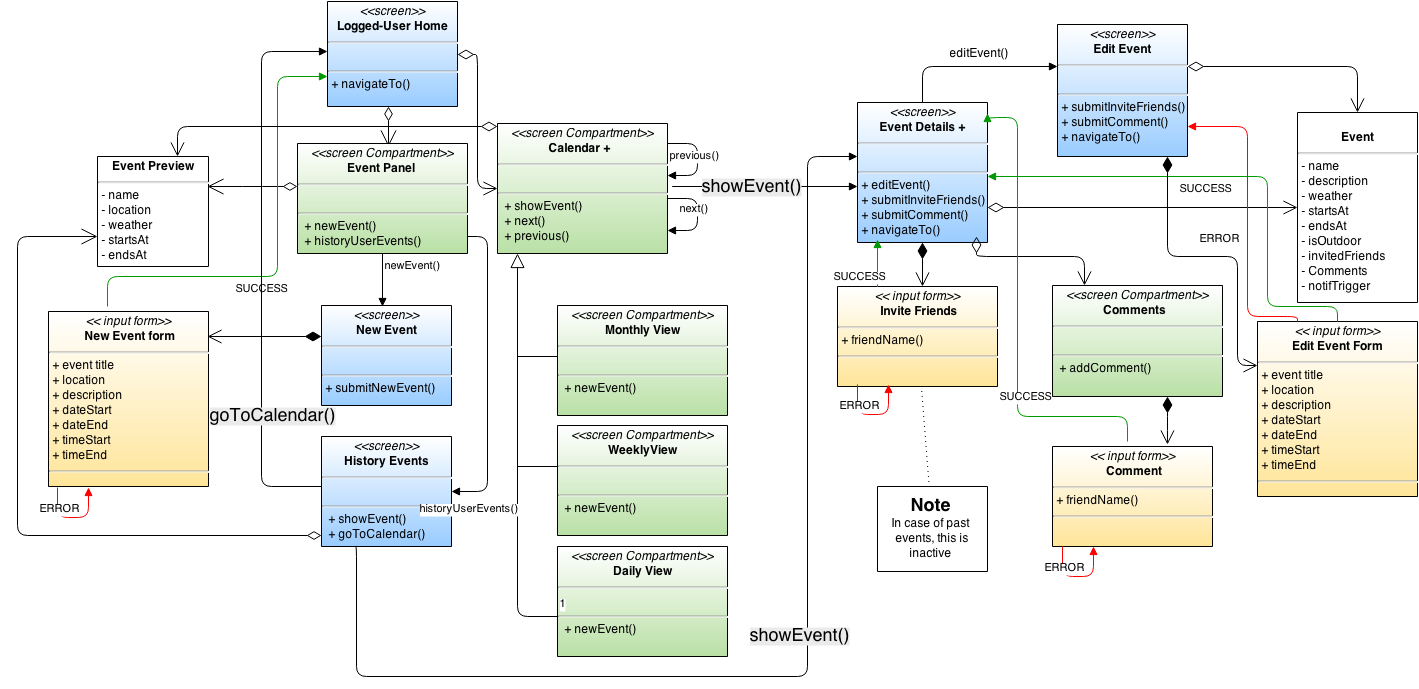
\includegraphics[scale=0.5]{event_management_UX}\\
\end{center}
\end{landscape}
\chapter{BCE Diagrams}
After having designed data model for the data layer and UX model for the web layer, it's now time to focus on the business logic, implemented in the so called business layer. As usual, before starting coding we have to give a preliminary design. \\
As already told before, the business layer contains both components that describe the data model (called JPA entities or Entity Beans) and components that describe business logic, implemented using EJB potentialities.\\

In order to design this part of document we decided to use the BCE model. It helps to understand Entity-Control-Boundary pattern, that is a simplification of the Model View Controller Pattern, if think that boundary can be mapped to the views, controls maps to the controller and entities mapped to the model. \\

As the UX model, also the BCE model is a UML model with some stereotypes: \\

- \textit{<<Entity>>} entities are objects representing system data. \\

- \textit{<<Boundary>>} boundaries are objects that interface with the system actors : UserInterfaces, DB Gateways, Proxies, ... . Boundaries are partially derived from the use cases and from some screens in the UX diagram\\

- \textit{<<Control>>} Controls are objects that mediate between boundary and entities. They orchestrate the execution of commands coming from the boundary by interacting with entity and boundary objects. Controls often correspond to use cases\\

In addition there are some rules that in a BCE model must be met: \\

- actors can only talk to boundary objects \\

- boundary objects can only talk to controllers and actors\\

- entity objects can only talk to controllers\\

- controllers can talk to boundary objects and entity objects, and the other controllers, but non to actors\\

\section{Entity Beans Model}
The Entity model is structured is a way that the set of JPA Entities (or Entity Beans) is directly linked to the conceptual model of data designed in chapter 4. \\
Anyway, these Entity Beans realizes such an abstraction that can be managed better in a Object Oriented application.  \\
As a matter of fact, to prevent the diagram to be too chaotic, in this part BCE diagram is split and just the an entity overview model is provided. \\
In order to simplify the notation, in this diagram \textit{getters and setters} method will be omitted.\\

\vspace{2cm}
\begin{center}
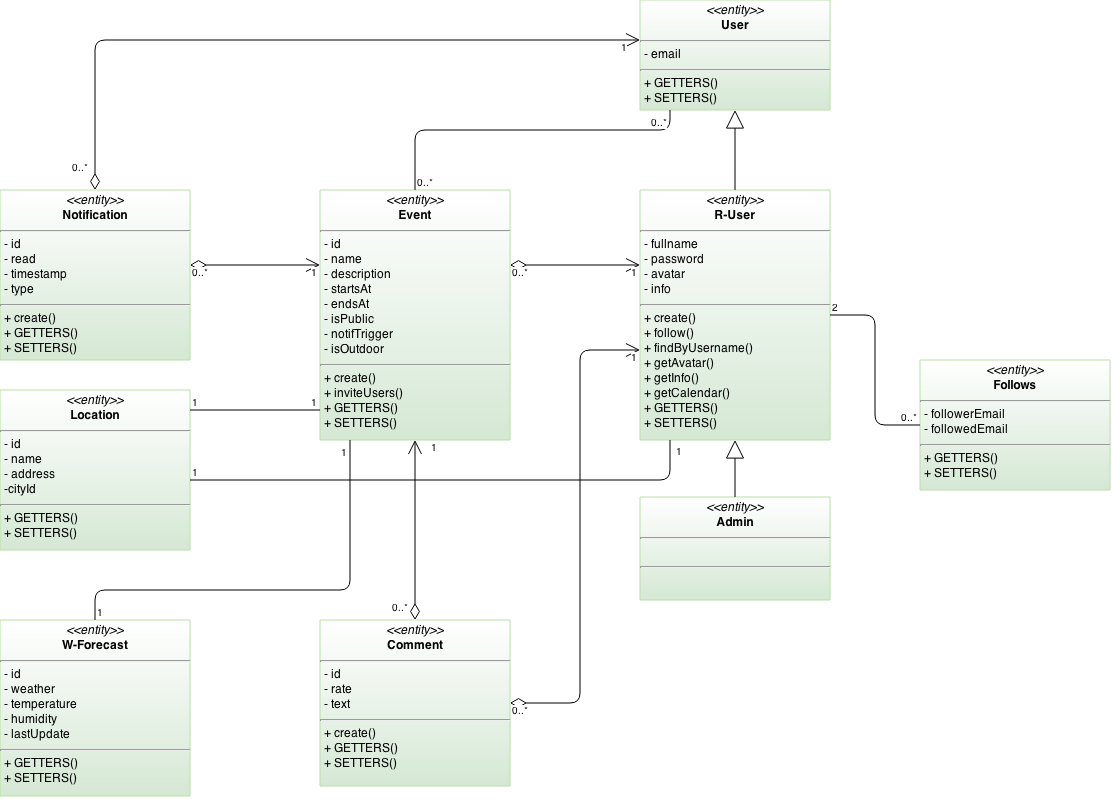
\includegraphics[scale=0.45]{entity}\\
\end{center}
\newpage
\section{Business Logic (EJB)}

In order to make further BCE diagrams clearer and more understandable, we want first to explain the relationship among UX screens and boundaries. There are some methods called \textit{showXXX()}, that refer to those methods whose goal is to display the correspondent screen. \\
\vspace{2cm}

\includegraphics[scale=0.45]{map_UX_bound}\\
\newpage
\subsection{Sign up and Log In}
In this BCE diagram there are three different boundaries: Not-Logged-User, Logged-User and Admin, which represent the interfaces that the three different types of users can reach. Each type of user has different functionalities and the system shows them personalized views.\\
Here we present a brief description of the used controllers:\\
- \textbf{ProfileManager:} 
	this component is in charge of manage users' profile data, both in case of sign up or update of 	profile information. It can verify the correctiveness of inserted data in the sign up phase and can 	create a new user in the system.\\
- \textbf{LoginManager:}
	this component manages the verification of data inserted in login fields. First of all it checks some parameters, like the password typed length, then can load the correspondent user finding it by e-mail address and check if the password typed matches with the stored one.\\
- \textbf{UserDataLoader:}
	this component has some methods that can load user's information after the login procedure, for example it can load user's calendar, its followers and new notifications.\\
	
Logged in user can be an administrator, and he has his own screen and therefore his own controller. It has few options that can modify system's behaviour.
For example the administrator can decide the frequency of weather update, he can establish if the system have to look for the weather report once a day, or maybe every 12 hours.\\

\vspace{2cm}
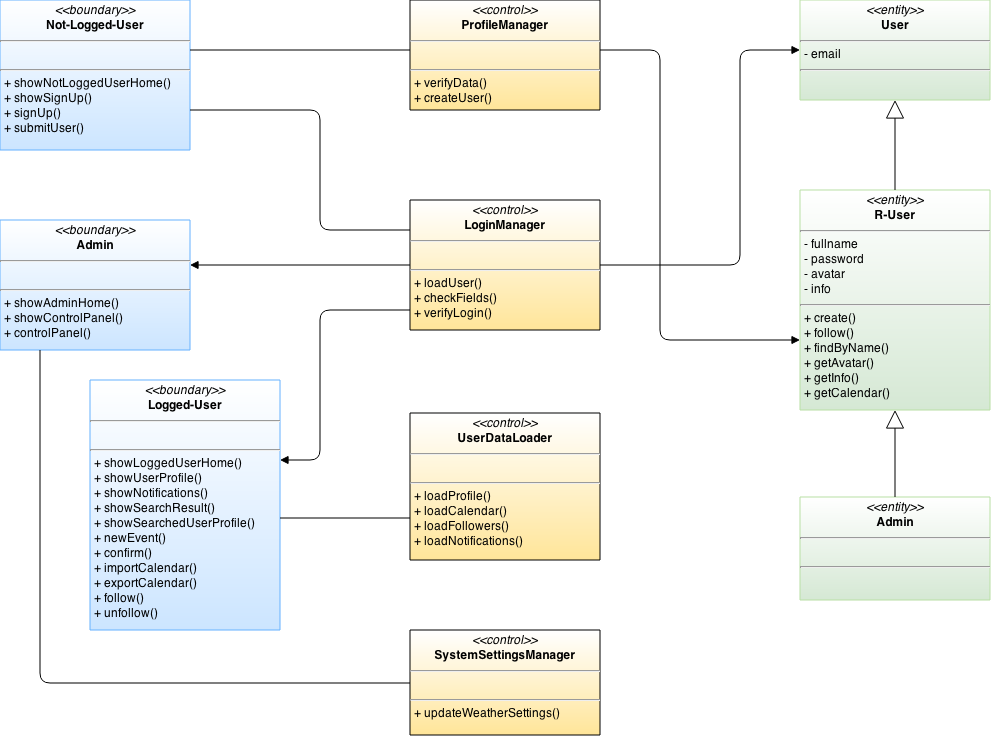
\includegraphics[scale=0.4]{signup_login}\\

\newpage
\subsection{Event management}
In this diagram we consider all the operations that a registered user can do on Events, for example creating a new event, or updating an existing one.
There are two different boundaries in this scenario:\\
- \textbf{LoggedUser: }contains all the user's screens, including his home page which is his calendar.\\
- \textbf{Event:} contains all the screens which refers to events, for example the Event Detail screen.\\

All the events functions are managed by three different controllers:\\
- \textbf{UserDataLoader: }besides loading user's profile information, this controller loads the user?s calendar (which is a set of events retrieved from persistent data) and also notifications that regard events.\\
- \textbf{EventManager: }this component manages the basic operations that an user can do on an event, for example creating a new one, but it also manages invitations allowing the user to send invitations, accept or decline.\\
- \textbf{WeatherForecastManager: }this controller is self managed, it doesn't need any interaction with boundaries, it is programmed to scan for up to dated weather conditions and check if there are bad weather conflicts with events in the schedule, then if it finds something,it creates a new notification for the user.\\

\vspace{2cm}
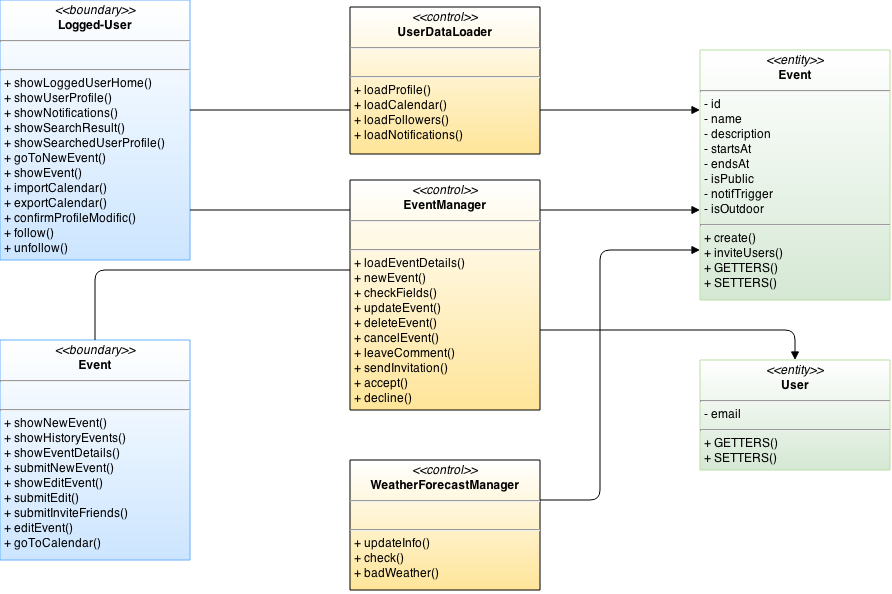
\includegraphics[scale=0.45]{user_events_BCE}\\

\newpage
\subsection{Social functions}
In this BCE diagram we focus on which kind of social operations a registered user can do, so the only boundary that appears is Logged User.\\
There are four different controllers:\\
- \textbf{UserDataLoader:}
	this component is activated when the user logs into the system, first of all it has to load all his informations in order to show the user's home page correctly, then it looks in the persistent data for some new notification to display into user's home page.\\
- \textbf{ProfileManager: }
	it allows user to update his own personal information, it interacts directly with the entity R-User in which information are stored and provides some methods to manipulate them.\\
- \textbf{SearchUserEngine: }
	this controller is a sort of search engine, which is able to find other users starting from a keyword, for example part of the username. It also provides a method that loads searched user's information to the search result page (note that this function is different from loadProfile() in UserDataLoader controller because you are not allowed to see all the information of another user, so we need two different procedures to distinguish among what data we have to load and what we have not).\\
- \textbf{FollowManager: }
	this component has only to manage follow relations between users. It interacts directly with the entity Follows, in which all the couples of Follower/Followed users are stored, it provides 	methods to add or remove a follower.\\
	
\vspace{2cm}
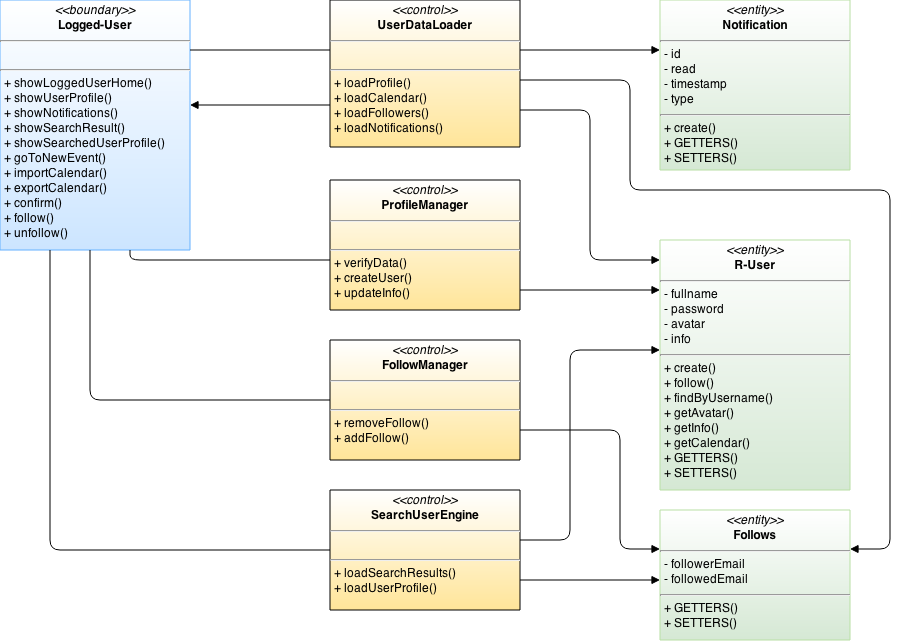
\includegraphics[scale=0.45]{user_social_BCE}\\

\chapter{Sequence Diagram}

In this section we will introduce some sequence diagrams to let readers better understand the dynamic of BCE diagrams designed above. This diagrams start again from the ones already studied in RASD document, but with more details. \\
Our goal is to underline the dynamic interaction between methods and class (beans). \\
For simplicity reasons, interactions between session bean and persistent layer are omitted. Also error situations are not took into account. \\

We will not design all possible sequence diagrams and neither all sequence diagrams provided in the RASD document, but just the most significative ones. 
We decided to design the following sequence diagrams : 
\begin{itemize}
\item{Log in}
\item{Sign up}
\item{Follow/Unfollow user}
\item{New Event}
\item{Friends Invitation}
\item{Profile updating}
\end{itemize}
\newpage
\section{Log in}
\vspace{2cm}
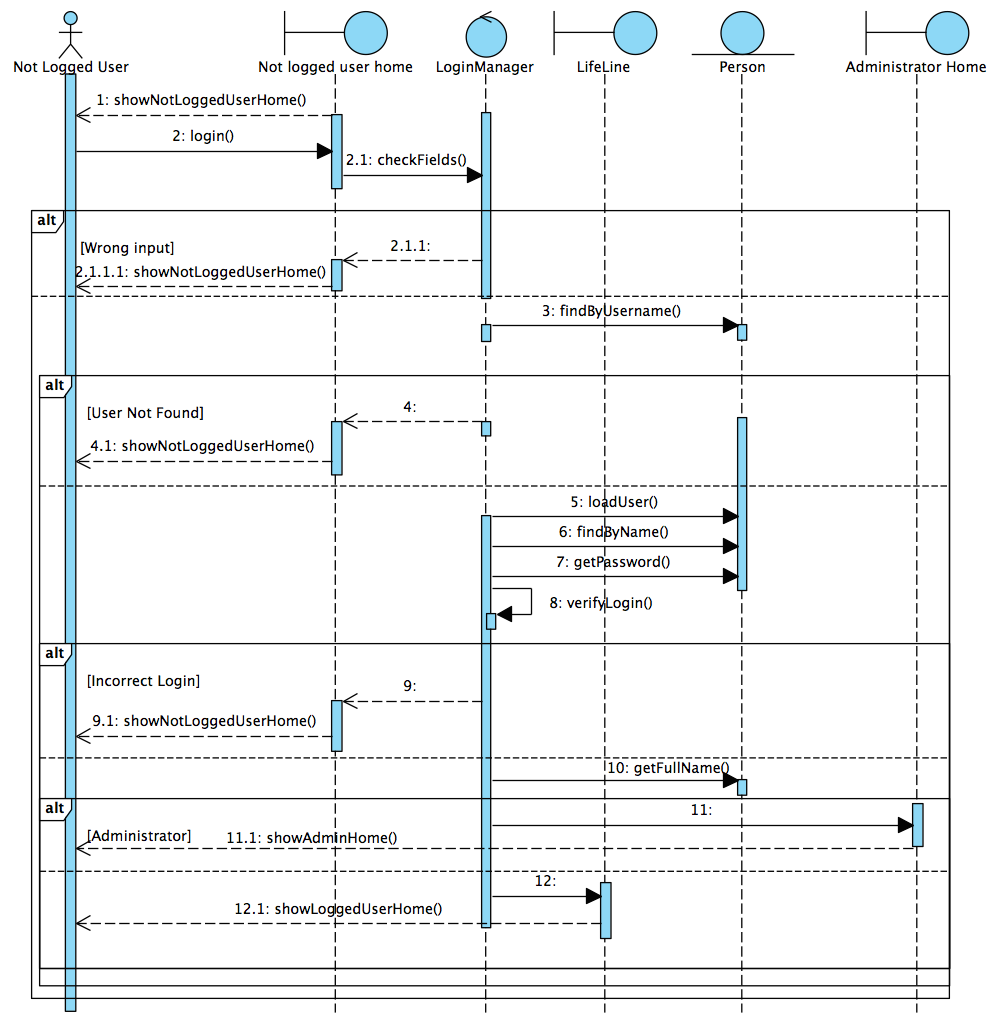
\includegraphics[scale=0.5]{Login_SD}
\newpage
\section{Sign up}
\vspace{2cm}
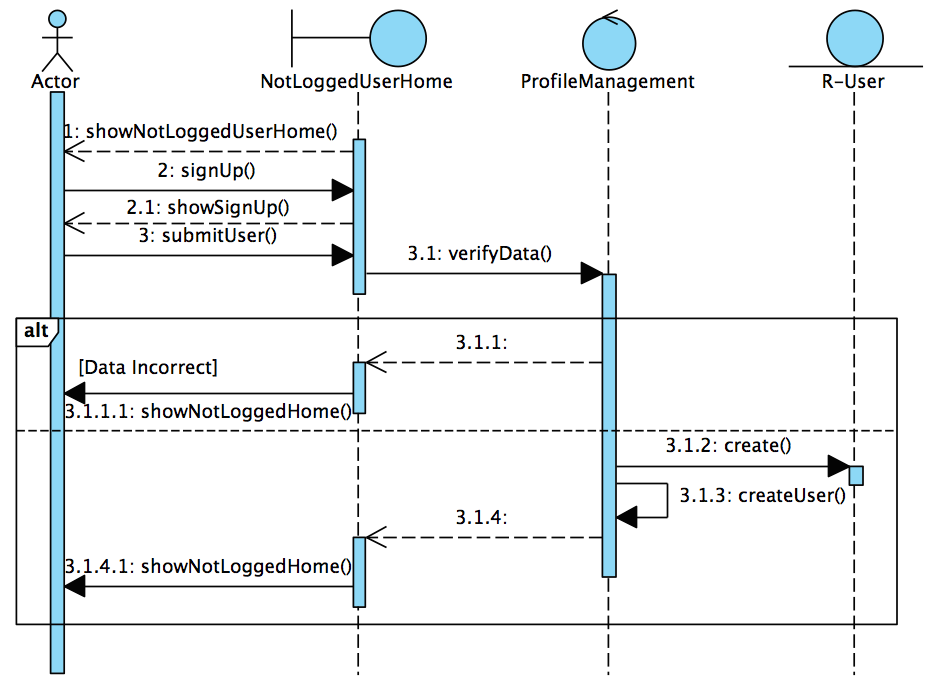
\includegraphics[scale=0.5]{signup_SD}
\newpage
\section{Follow/Unfollow user}
\vspace{2cm}
\includegraphics[scale=0.5]{follow_SD}
\newpage
\section{New Event}
\vspace{2cm}
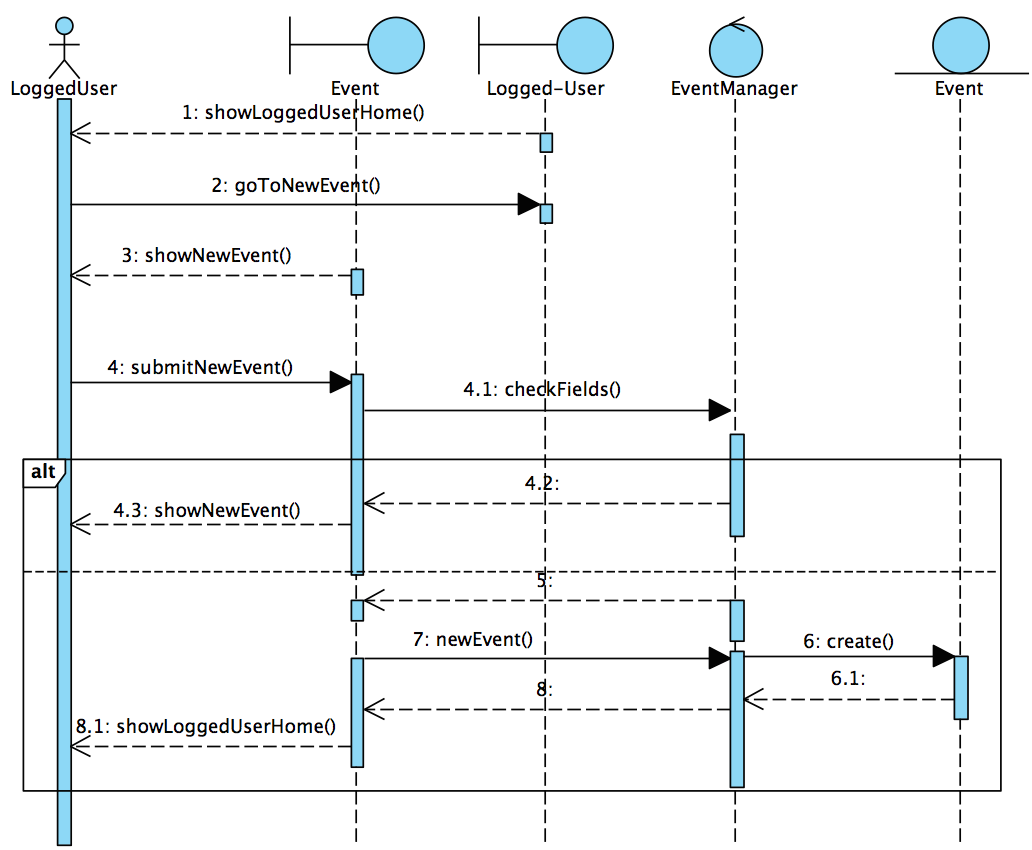
\includegraphics[scale=0.45]{newevent_SD}
\newpage
\section{Friends Invitation}
\vspace{2cm}
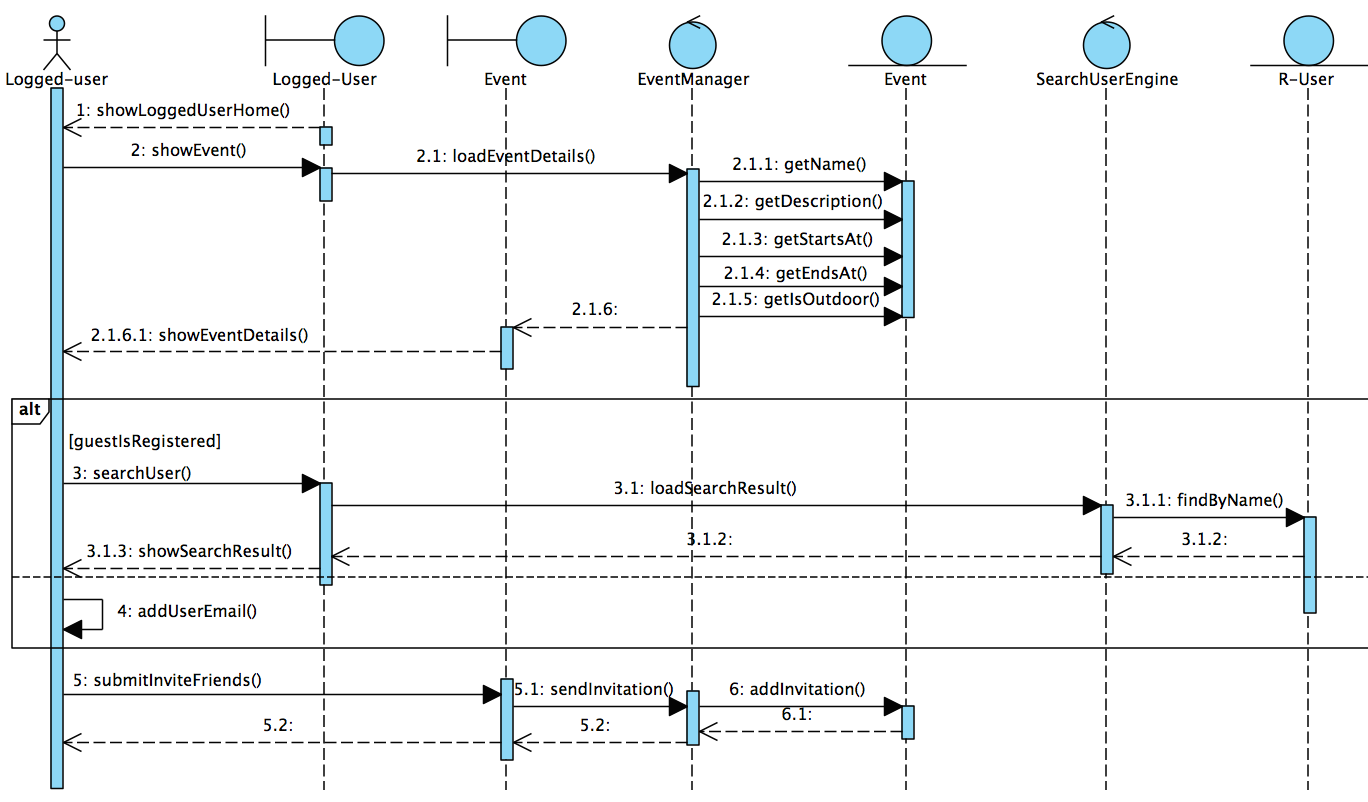
\includegraphics[width=18cm,height=13cm]{friendsinvitation_SD}
\newpage
\section{Profile updating}
\vspace{2cm}
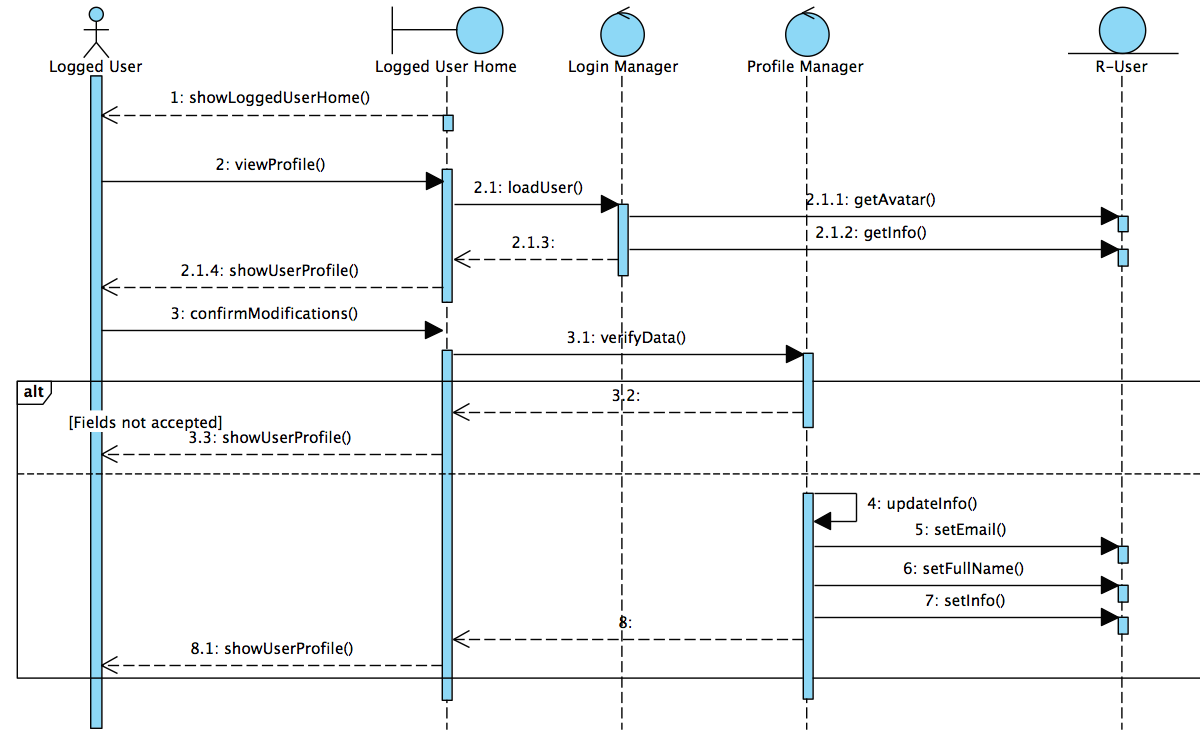
\includegraphics[width=18cm,height=13cm]{updateInfo_SD}
\newpage

\chapter{Used Tools}
\begin{itemize}
\item{LaTeX for writing the document}
\item{MySQLWorkBench for designing logical model}
\item{Keynote for designing conceptual ER model}
\item{Online application draw.io for designing UX and BCE diagrams}
\item{Visual Paradigm for designing sequence diagrams}
\end{itemize}
\chapter{References}
- SE2 teacher Mirandola's lecture slides\\
- SE2 teacher Tamburri's lecture slides\\
- \textit{https://www.oasis-open.org/committees/download.php/24846/Example-SoftwareDesignDocument-LegalXMLUtility.pdf}\\
- \textit{$http://en.wikipedia.org/wiki/Software\_design\_document$}\\
- \textit{$http://cs.kennesaw.edu/snorth/CS\_SE/SDD\_Template.pdf$}\\
- \textit{$https://mdn.mozillademos.org/files/4291/client-server.png$}\\
- DD example from past year\\

\end{document}
